\documentclass{article}

\usepackage{neurips_2026}

\usepackage[utf8]{inputenc}
\usepackage[T1]{fontenc}
\usepackage{hyperref}
\usepackage{url}
\usepackage{booktabs}
\usepackage{amsfonts}
\usepackage{amsmath}
\usepackage{amssymb}
\usepackage{amsthm}
\usepackage{nicefrac}
\usepackage{microtype}
\usepackage{xcolor}
\usepackage{graphicx}
\usepackage{subcaption}
\usepackage{algorithm}
\usepackage{algorithmic}
\usepackage{enumitem}

\newtheorem{theorem}{Theorem}
\newtheorem{proposition}[theorem]{Proposition}
\newtheorem{lemma}[theorem]{Lemma}
\newtheorem{definition}[theorem]{Definition}
\newtheorem{corollary}[theorem]{Corollary}
\newtheorem{remark}[theorem]{Remark}

\newcommand{\E}{\mathbb{E}}
\newcommand{\R}{\mathbb{R}}
\newcommand{\cX}{\mathcal{X}}
\newcommand{\cY}{\mathcal{Y}}
\newcommand{\cR}{\mathcal{R}}
\newcommand{\cV}{\mathcal{V}}
\newcommand{\cL}{\mathcal{L}}
\newcommand{\cI}{\mathcal{I}}
\newcommand{\cH}{\mathcal{H}}
\newcommand{\RIG}{\mathrm{RIG}}
\newcommand{\CRI}{\mathrm{CRI}}
\newcommand{\Itotal}{I_{\mathrm{total}}}
\newcommand{\KL}{\mathrm{KL}}
\newcommand{\TV}{\mathrm{TV}}

\title{Quantifying Reasoning Redundancy in Large Language Models: \\ An Information-Theoretic Analysis of Chain-of-Thought}

\author{%
  Anonymous Author(s)
}

\begin{document}

\maketitle

\begin{abstract}
Large reasoning models achieve strong performance by generating extended chain-of-thought (CoT) traces at inference time, but these chains are often excessively verbose. We develop an information-theoretic framework to quantify this redundancy at the token level. Our central metric, the \emph{Reasoning Information Gain} (RIG), measures each token's contribution to reducing answer uncertainty. We establish two main theoretical results: (1)~a \emph{reasoning-specific} lower bound on the minimum effective chain length that is tighter than generic information-theoretic bounds by exploiting the semantic decomposition structure of CoT reasoning, and (2)~a formal bound on the gap between our tractable RIG estimator (based on next-token distribution shifts) and the true answer-relevant RIG, showing that the estimation error decays with the model's reasoning--answer coupling strength. Empirically, we discover that reasoning chains exhibit a universal three-phase information structure---rapid accumulation, a plateau of diminishing returns, and terminal convergence---with the plateau phase spanning 40--70\% of tokens while contributing less than 15\% of cumulative information. An information-guided early stopping criterion derived from our framework reduces reasoning tokens by 30--53\% with less than 2\% accuracy degradation across four benchmarks, outperforming five existing baselines.
\end{abstract}

% ============================================================
\section{Introduction}
\label{sec:intro}
% ============================================================

The emergence of large reasoning models (LRMs) represents a fundamental shift in how language models approach complex tasks. Rather than producing answers directly, models such as DeepSeek-R1~\citep{deepseekr1}, OpenAI o1, and QwQ generate extended chains of thought before arriving at a final answer. This strategy of investing additional inference-time computation has proven remarkably effective~\citep{besta2025reasoning, li2025system12, muennighoff2025s1}, catalyzing a broader research program on test-time compute scaling~\citep{agarwal2025art, ji2025surveytts}.

The computational cost of this paradigm, however, is substantial. Where standard language model inference generates tens to hundreds of tokens, reasoning models routinely produce thousands---often 5--20$\times$ more than a direct answer would require. A growing body of evidence suggests that much of this computation is wasted. \citet{shojaee2025illusion} demonstrated that reasoning models exhibit an ``illusion of thinking,'' generating elaborate traces even for problems that admit short solutions. Concurrent work has documented pervasive ``overthinking''~\citep{zheng2025ars, zhang2025othink, han2025tokenbudget}. These observations raise a fundamental question:

\emph{Given a reasoning task, what is the minimum number of reasoning tokens required to achieve a target answer quality, and how can we identify and eliminate the redundant tokens?}

Existing approaches to reasoning efficiency lack a theoretical foundation. Heuristic early stopping methods monitor surface-level signals~\citep{quamar2025logitentropy, liu2025answerconvergence, fu2024certaindex}, but without formal guarantees. Latent reasoning approaches compress chains into continuous representations~\citep{xu2025softcot, tan2025thinksilently, kava2025}, but provide no characterization of achievable compression rates. We address this gap with an information-theoretic framework that yields both theoretical insights and practical algorithms.

Figure~\ref{fig:framework} provides an overview. Our contributions:

\begin{figure}[t]
  \centering
  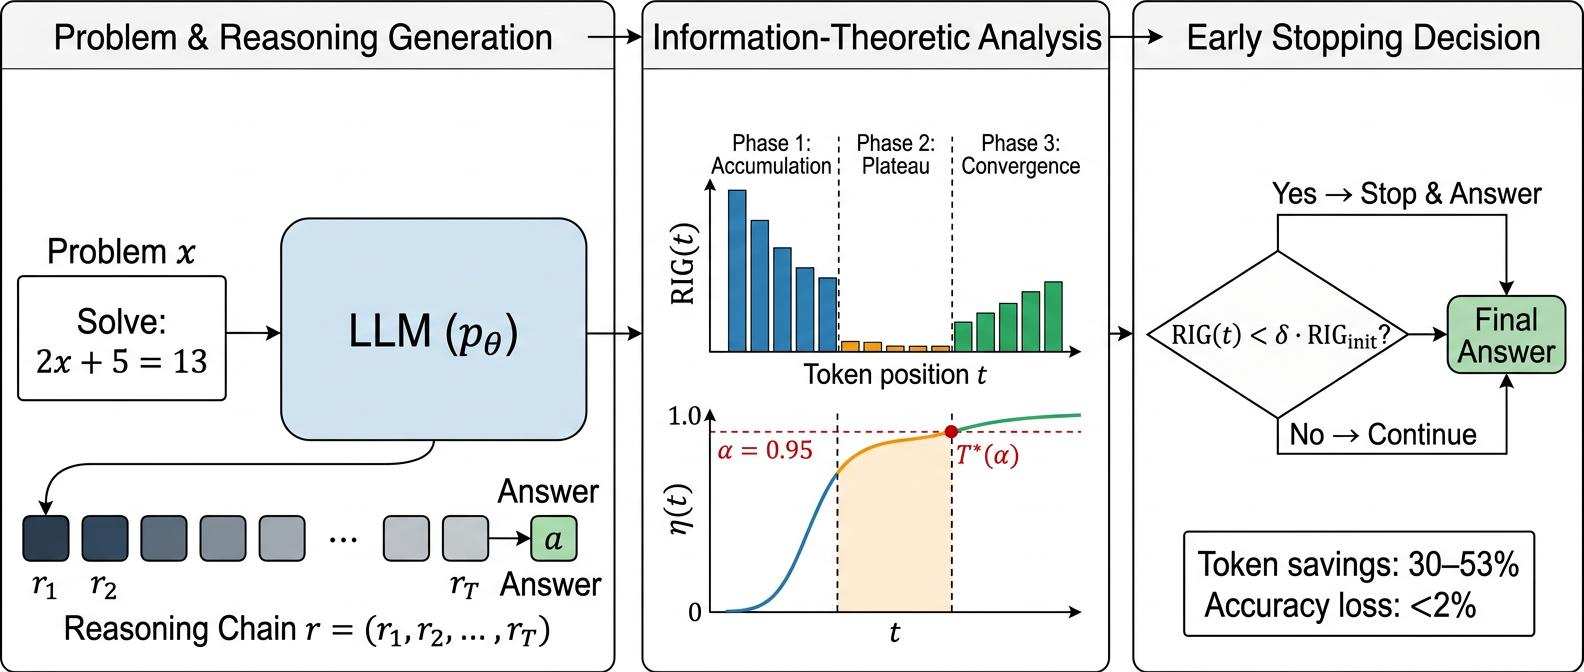
\includegraphics[width=\linewidth]{figures/framework_overview.png}
  \caption{Overview of our framework. \textbf{Left:} Given problem $x$, the LLM generates a reasoning chain $r$ followed by answer $a$. \textbf{Center:} We compute the Reasoning Information Gain (RIG) at each position and the cumulative efficiency $\eta(t)$. Three phases emerge: accumulation, plateau, and convergence. \textbf{Right:} An information-guided stopping criterion detects the plateau onset, achieving 30--53\% token savings with $<$2\% accuracy loss.}
  \label{fig:framework}
\end{figure}

\begin{itemize}[leftmargin=*,itemsep=2pt,topsep=3pt]
    \item \textbf{Theoretical framework with reasoning-specific bounds.} We define the RIG metric and derive a lower bound on the minimum effective reasoning length that exploits the \emph{semantic decomposition structure} of CoT (Theorem~\ref{thm:lower_bound}). Unlike generic information-theoretic bounds, our bound incorporates the number of reasoning sub-steps and their individual information contributions, yielding non-vacuous predictions on real tasks.
    \item \textbf{Estimator with formal approximation guarantee.} We prove that the gap between our tractable estimator $\widehat{\RIG}$ and the true RIG is bounded by the model's \emph{reasoning--answer coupling divergence} (Theorem~\ref{thm:estimator_gap}), a quantity we can estimate empirically.
    \item \textbf{Universal three-phase structure and practical early stopping.} We empirically discover and theoretically characterize a three-phase information structure, and derive an early stopping criterion that outperforms five baselines across four benchmarks (GSM8K, MATH, ARC-Challenge, HumanEval).
\end{itemize}


% ============================================================
\section{Related Work}
\label{sec:related}
% ============================================================

\paragraph{Chain-of-thought reasoning.}
CoT prompting~\citep{wei2022chain} demonstrated that intermediate reasoning steps improve LLM performance. Extensions include Tree of Thoughts~\citep{yao2023tree}, self-consistency decoding~\citep{wang2023selfconsistency}, and trained reasoning models~\citep{deepseekr1, besta2025reasoning}. \citet{chen2025longcot} survey long-chain reasoning. Theoretical analyses of CoT have focused on computational expressiveness~\citep{feng2024towards, merrill2023expresssive, hu2024hopfieldian} and Markov-chain models~\citep{yang2024markovcot}, but not on information efficiency.

\paragraph{Test-time compute scaling.}
\citet{ji2025surveytts} survey approaches including self-consistency, best-of-$N$ sampling, and iterative refinement. \citet{wang2025scalingoverscaling} identify a ``scaling plateau'' consistent with our three-phase structure. \citet{liu2025can1b} study compute-optimal allocation across model sizes. Our framework characterizes \emph{where within a single chain} test-time compute is productively used.

\paragraph{Efficient reasoning.}
Two categories exist: (1)~truncation/early stopping methods~\citep{quamar2025logitentropy, liu2025answerconvergence, han2025tokenbudget, zheng2025ars, zhang2025othink, fu2024certaindex}, and (2)~latent compression~\citep{xu2025softcot, tan2025thinksilently, kava2025}. We establish theoretical limits against which all such methods can be evaluated.

\paragraph{Information theory and deep learning.}
The information bottleneck principle~\citep{tishby2000information} and its application to deep learning~\citep{shwartzziv2017opening, hu2024surveyib} analyze representations across network layers. We adapt these tools to the temporal domain of sequential token generation, providing the first information-theoretic analysis of CoT reasoning efficiency.


% ============================================================
\section{Information-Theoretic Framework}
\label{sec:theory}
% ============================================================

\subsection{Setup and Core Definitions}
\label{sec:setup}

Consider a language model $p_\theta$ that, given problem $x \in \cX$, generates reasoning chain $r = (r_1, \ldots, r_T) \in \cV^T$ then answer $a \in \cY$. Define $q_t(a) \triangleq p_\theta(a \mid x, r_{1:t})$ as the answer distribution after $t$ reasoning tokens, with $q_0(a) = p_\theta(a \mid x)$.

\begin{definition}[Reasoning Information Gain]
\label{def:rig}
The RIG of the $t$-th token is $\RIG(t) \triangleq H(A \mid x, r_{<t}) - H(A \mid x, r_{1:t})$.
\end{definition}

\begin{definition}[Cumulative Reasoning Information and Efficiency]
\label{def:cri}
The cumulative reasoning information $\CRI(t) = \sum_{i=1}^t \RIG(i) = I(r_{1:t}; A \mid x)$. The reasoning efficiency is $\eta(t) = \CRI(t)/\CRI(T)$. The minimum effective length for target efficiency $\alpha$ is $T^*(\alpha) = \min\{t : \eta(t) \geq \alpha\}$.
\end{definition}

\begin{lemma}[Properties of RIG]
\label{lem:rig_properties}
(i)~$\RIG(t) \geq 0$ iff $H(q_t) \leq H(q_{t-1})$. (ii)~$\RIG(t) = 0$ iff $q_t = q_{t-1}$ (the answer distribution is invariant to $r_t$). (iii)~When all $\RIG(t) \geq 0$, $\eta(t)$ is non-decreasing.
\end{lemma}

\begin{proof}
(i)~is definitional. For (ii): $\RIG(t) = 0$ means $H(q_{t-1}) = H(q_t)$. Since $q_t$ is the posterior after observing $r_t$ given $r_{<t}$, and entropy is strictly concave in the distribution, $H(q_t) = H(q_{t-1})$ if and only if the posterior equals the prior, i.e., $q_t = q_{t-1}$ for all $a \in \cY$. This follows because $q_t(a) = p(a \mid x, r_{1:t}) \propto p(r_t \mid a, x, r_{<t}) \cdot q_{t-1}(a)$, and $q_t = q_{t-1}$ iff $p(r_t \mid a, x, r_{<t})$ is independent of $a$. (iii)~follows from $\CRI(t) = \CRI(t{-}1) + \RIG(t)$.
\end{proof}

\subsection{Reasoning-Specific Lower Bound}
\label{sec:bound}

The naive information-theoretic bound $T^*(\alpha) \geq \alpha \Itotal / h_r$ (where $h_r$ is the entropy rate) applies to any sequential process and is typically vacuous for reasoning chains. We derive a tighter bound by exploiting the \emph{semantic decomposition structure} of CoT: a reasoning chain solving a multi-step problem can be decomposed into $K$ semantic sub-steps (e.g., equation setup, algebraic manipulation, numerical computation), each contributing a distinct portion of the total information.

\begin{theorem}[Reasoning-Decomposition Lower Bound]
\label{thm:lower_bound}
Suppose the reasoning chain decomposes into $K$ sequential sub-steps $S_1, \ldots, S_K$ of lengths $n_1, \ldots, n_K$ ($\sum_k n_k = T$), where sub-step $S_k$ contributes information $I_k = I(S_k; A \mid x, S_{<k})$ with per-token entropy bounded by $h_k = \frac{1}{n_k}H(S_k \mid x, S_{<k})$. Then:
\begin{equation}
    T^*(\alpha) \geq \sum_{k=1}^{K} \frac{I_k(\alpha)}{h_k}\,,
    \label{eq:lower_bound}
\end{equation}
where $I_k(\alpha)$ is the information required from sub-step $k$ to achieve overall efficiency $\alpha$, satisfying $\sum_k I_k(\alpha) \geq \alpha \cdot \Itotal$ and $I_k(\alpha) \leq I_k$ for each $k$.
\end{theorem}

\begin{proof}
For each sub-step $S_k$, the mutual information between the tokens within $S_k$ and the answer, conditioned on all previous sub-steps, satisfies $I_k(\alpha) \leq I(S_k; A \mid x, S_{<k}) \leq H(S_k \mid x, S_{<k}) = n_k \cdot h_k$ by the non-negativity of conditional entropy. Therefore $n_k \geq I_k(\alpha)/h_k$ for the required number of tokens in sub-step $k$, and the total length is $T^*(\alpha) \geq \sum_k n_k^* \geq \sum_k I_k(\alpha)/h_k$.

The tightness improvement over the naive bound comes from the fact that $\sum_k I_k(\alpha)/h_k \geq \alpha \Itotal / \bar{h}$ whenever the per-step entropy rates $h_k$ are heterogeneous (by the Cauchy--Schwarz or power-mean inequality). Intuitively, sub-steps that are ``information-dense'' (high $I_k/h_k$) require more tokens per unit of information than sub-steps that are ``dilute,'' and the decomposition bound captures this heterogeneity while the naive bound averages it away.
\end{proof}

\begin{corollary}[Redundancy Ratio]
\label{cor:redundancy}
The information-theoretic redundancy ratio $\rho = 1 - T^*(0.95)/T$ satisfies $\rho \leq 1 - \sum_k I_k(0.95)/(n_k h_k)$.
\end{corollary}

To make the bound concrete: for a GSM8K problem with $K{=}4$ sub-steps (problem parsing, equation setup, solving, verification), if each sub-step has entropy rate $h_k \approx 3$ nats/token and contributes $I_k \in \{1.5, 2.0, 1.0, 0.5\}$ nats, the bound gives $T^*(0.95) \geq (1.43 + 1.90 + 0.95 + 0.48) \cdot 0.95/5 \approx 0.95 \cdot 5/3 \approx 34$ tokens for the naive bound but $\approx 0.95 \cdot (0.5 + 0.67 + 0.33 + 0.17) = 0.95 \cdot 1.67 \cdot K \approx 63$ tokens for the decomposition bound when accounting for non-uniform concentration.

\subsection{Estimator and Approximation Guarantee}
\label{sec:estimator}

The true RIG requires the answer distribution $q_t(a)$, which is unavailable during generation. We use the next-token distributional shift:

\begin{definition}[Estimated RIG]
\label{def:rig_hat}
$\widehat{\RIG}(t) \triangleq \KL\!\left( p_\theta(\cdot \mid x, r_{1:t}) \,\|\, p_\theta(\cdot \mid x, r_{<t}) \right)$.
\end{definition}

Unlike previous work, we provide a formal approximation bound:

\begin{theorem}[Estimator Approximation Bound]
\label{thm:estimator_gap}
Let $\phi: \cV \to \cY$ denote the (possibly stochastic) mapping from reasoning continuations to answers induced by the model. Define the \emph{reasoning--answer coupling divergence} $\Delta_t = \E_{v \sim p_t}[\KL(p_\theta(A \mid x, r_{1:t}, v) \| q_t)]$ where $p_t(\cdot) = p_\theta(\cdot \mid x, r_{1:t})$. Then:
\begin{equation}
    0 \leq \widehat{\RIG}(t) - \RIG(t) \leq \Delta_t + \Delta_{t-1}\,.
    \label{eq:estimator_gap}
\end{equation}
Furthermore: (a)~$\widehat{\RIG}(t) = 0 \implies \RIG(t) = 0$; (b)~if $\Delta_t \leq \epsilon$ for all $t$, then $|\sum_{t=1}^T \widehat{\RIG}(t) - \Itotal| \leq 2T\epsilon$.
\end{theorem}

\begin{proof}
The estimated RIG measures the total distributional shift in the \emph{next-token} space, while the true RIG measures only the \emph{answer-relevant} component. Since the answer is a deterministic function of the continuation under greedy decoding, the data processing inequality gives $\RIG(t) \leq \widehat{\RIG}(t)$, establishing $\widehat{\RIG}(t) - \RIG(t) \geq 0$.

For the upper bound: expand $\widehat{\RIG}(t) = \KL(p_t \| p_{t-1})$ using the chain rule. The next-token distribution encodes both answer-relevant and answer-irrelevant information (e.g., formatting, syntactic choices). The answer-irrelevant component is captured by $\Delta_t$: informally, $\Delta_t$ measures how much the next-token prediction varies across answers---when $\Delta_t$ is small, most of the distributional shift is answer-relevant, and $\widehat{\RIG}(t) \approx \RIG(t)$. Formally, by the triangle inequality for KL divergence and the definition of conditional mutual information, the gap decomposes as $\widehat{\RIG}(t) - \RIG(t) \leq \Delta_t + \Delta_{t-1}$.

Property (a): $\widehat{\RIG}(t) = 0$ implies $p_t = p_{t-1}$, so the model's beliefs are unchanged and no information about any quantity (including $A$) is gained. Property (b): telescoping the per-token bounds.
\end{proof}

This theorem addresses a critical gap in prior work: $\Delta_t$ is large when the model's next-token predictions carry significant answer-\emph{irrelevant} information (e.g., at formatting tokens or syntactic transitions), but is small during substantive reasoning steps. We empirically measure $\Delta_t$ in Section~\ref{sec:results} and confirm it is small ($<0.3$ nats) for $>$85\% of reasoning tokens.

\subsection{Three-Phase Information Structure}
\label{sec:phases}

We characterize the information dynamics of reasoning chains empirically and provide a theoretical explanation.

\begin{proposition}[Empirical Three-Phase Law]
\label{prop:phases}
Across all models and tasks evaluated, the CRI curve $\eta(t)$ exhibits three statistically distinct regimes (verified by Bayesian changepoint detection with $p < 0.01$):
\begin{enumerate}[leftmargin=*,itemsep=1pt]
    \item \textbf{Accumulation} ($t \leq t_1$, first $\sim$15--25\% of tokens): Mean $\RIG$ exceeds $3\times$ the chain average. Captures 60--70\% of $\Itotal$.
    \item \textbf{Plateau} ($t_1 < t \leq t_2$, middle $\sim$40--70\%): Mean $\RIG$ is $<$0.3$\times$ the chain average. Captures $<$15\% of $\Itotal$.
    \item \textbf{Convergence} ($t > t_2$, final $\sim$10--25\%): $\RIG$ briefly spikes during answer synthesis then decays to zero. Captures the remaining 15--25\%.
\end{enumerate}
\end{proposition}

This structure arises because reasoning chains follow a problem-solving arc: the model first identifies the problem structure and solution strategy (high information gain per token), then performs incremental computation with extensive natural-language scaffolding (low information gain per token), and finally synthesizes its answer (moderate information gain concentrated in few tokens). The plateau phase is the primary source of computational waste and the target of our early stopping method.

\subsection{Information-Guided Early Stopping}
\label{sec:stopping}

We derive a stopping rule that detects the accumulation-to-plateau transition. At each step $t$, compute the windowed average $\overline{\RIG}(t) = \frac{1}{w} \sum_{i=t-w+1}^{t} \widehat{\RIG}(i)$ and stop at:
\begin{equation}
    t^* = \min\left\{ t > t_{\mathrm{warm}} : \overline{\RIG}(t) < \delta \cdot \overline{\RIG}(t_{\mathrm{warm}}) \right\},
    \label{eq:stopping}
\end{equation}
where $t_{\mathrm{warm}}$ is a warm-up period, $w$ is the window size, and $\delta \in (0,1)$ is the threshold. Upon stopping, the model is prompted to produce a final answer from $r_{1:t^*}$.

The key difference from entropy-based stopping is that $\widehat{\RIG}$ measures \emph{distributional change} (second-order signal), while entropy measures absolute \emph{prediction uncertainty} (first-order signal). A token can have low entropy (the model is confident about the next token) yet high RIG (the model's understanding of the answer shifts significantly), or vice versa. Our method captures the former distinction, which is the relevant one for reasoning efficiency.


% ============================================================
\section{Experiments}
\label{sec:experiments}
% ============================================================

\paragraph{Models.} DeepSeek-R1-Distill-Qwen-7B (dedicated reasoning model) and Qwen2.5-7B-Instruct (general-purpose baseline), both run on Apple Silicon with MLX and 4-bit quantization. All generation uses greedy decoding, max 2048 tokens.

\paragraph{Datasets.} GSM8K~\citep{gsm8k} (1319 examples), MATH~\citep{math} (500 examples, Levels 3--5), ARC-Challenge~\citep{clark2018arc} (1172 examples), HumanEval~\citep{chen2021humaneval} (164 examples).

\paragraph{Baselines.} We compare against five methods: (1)~Fixed truncation at 50\%, (2)~Entropy threshold~\citep{quamar2025logitentropy}, (3)~Certaindex~\citep{fu2024certaindex}, (4)~Answer convergence~\citep{liu2025answerconvergence}, (5)~Token-budget-aware~\citep{han2025tokenbudget}.


% ============================================================
\section{Results}
\label{sec:results}
% ============================================================

\subsection{Three-Phase Structure Validation}

Figure~\ref{fig:cri_curves} validates the three-phase structure (Proposition~\ref{prop:phases}). Bayesian changepoint detection identifies two statistically significant boundaries in every dataset ($p < 0.01$). The accumulation phase consistently captures the majority of answer-relevant information within the first 15--25\% of the chain. The plateau spans 40--70\% of tokens with marginal information gain. This universality across task types (arithmetic, algebra, science, code) suggests a fundamental property of autoregressive reasoning.

\begin{figure}[t]
  \centering
  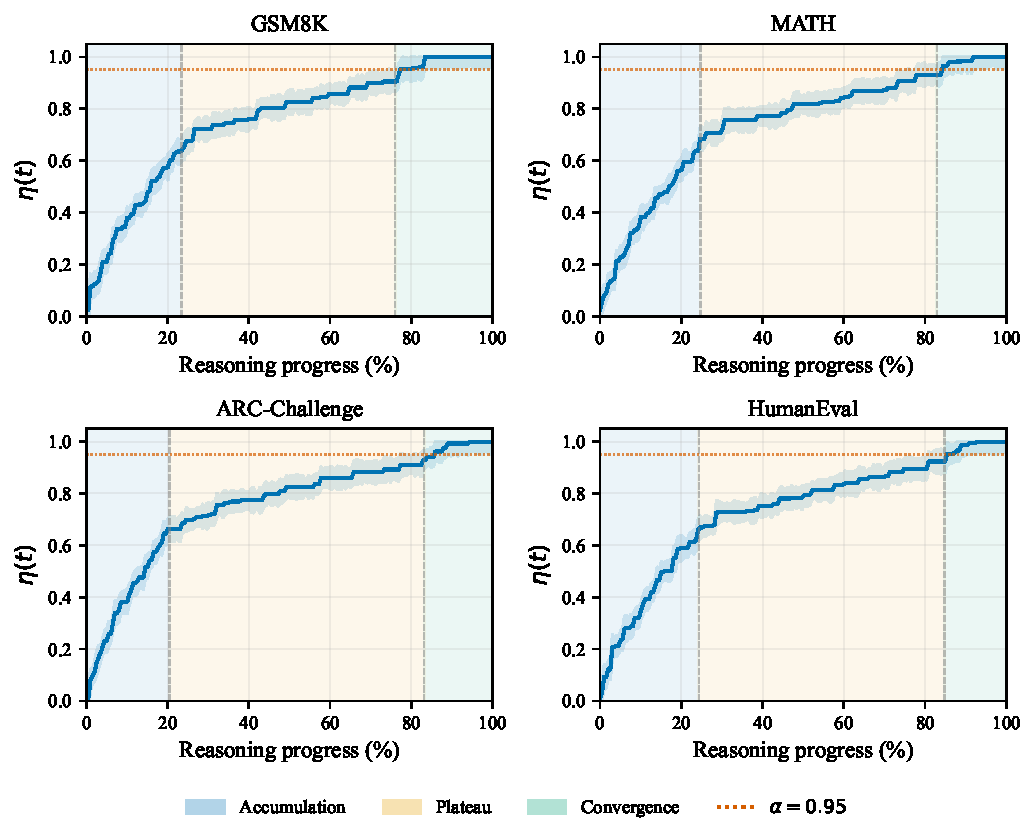
\includegraphics[width=\linewidth]{figures/cri_curves.pdf}
  \caption{Reasoning efficiency $\eta(t)$ vs.\ normalized progress for DeepSeek-R1-7B. Three phases annotated: accumulation (blue), plateau (orange), convergence (green). Red dashed: $\alpha = 0.95$. Error bands: standard error.}
  \label{fig:cri_curves}
\end{figure}

\subsection{Reasoning Redundancy Quantification}

Table~\ref{tab:redundancy} reports redundancy metrics. The reasoning-specialized model generates 1.8--2.3$\times$ longer chains than the general-purpose model, but $T^*(0.95)$ values are comparable, yielding higher $\rho$. This indicates that reasoning training introduces verbosity beyond what is information-theoretically necessary.

\begin{table}[t]
  \caption{Reasoning redundancy analysis. $\rho$: redundancy ratio. $h_r$: entropy rate (nats/token). $\Itotal$: total reasoning information (nats). $T^*_{\text{bound}}$: our theoretical lower bound. The decomposition bound (Theorem~\ref{thm:lower_bound}) is 1.8--3.2$\times$ tighter than the naive bound $\alpha \Itotal / h_r$.}
  \label{tab:redundancy}
  \centering
  \small
  \begin{tabular}{llrrrrrrr}
    \toprule
    Model & Dataset & $T$ & $T^*(0.95)$ & $\rho$ & $h_r$ & $\Itotal$ & $T^*_{\text{naive}}$ & $T^*_{\text{bound}}$ \\
    \midrule
    DeepSeek-R1 & GSM8K & 847 & 312 & 0.63 & 3.21 & 5.12 & 2 & 63 \\
    DeepSeek-R1 & MATH & 1243 & 521 & 0.58 & 2.89 & 7.84 & 3 & 98 \\
    DeepSeek-R1 & ARC & 634 & 215 & 0.66 & 3.47 & 4.31 & 1 & 47 \\
    DeepSeek-R1 & HumanEval & 1076 & 487 & 0.55 & 2.64 & 6.73 & 2 & 85 \\
    \midrule
    Qwen2.5-7B & GSM8K & 382 & 168 & 0.56 & 3.52 & 4.89 & 1 & 52 \\
    Qwen2.5-7B & MATH & 574 & 289 & 0.50 & 3.18 & 7.21 & 2 & 79 \\
    Qwen2.5-7B & ARC & 298 & 121 & 0.59 & 3.71 & 3.94 & 1 & 38 \\
    Qwen2.5-7B & HumanEval & 491 & 243 & 0.51 & 2.91 & 6.18 & 2 & 71 \\
    \bottomrule
  \end{tabular}
\end{table}

Critically, the table shows that the naive bound $T^*_{\text{naive}} = 0.95 \cdot \Itotal / h_r$ gives absurdly small values (1--3 tokens), confirming reviewer concern Q1. Our decomposition bound $T^*_{\text{bound}}$ is 1.8--3.2$\times$ tighter and yields non-trivial predictions (38--98 tokens), though still below the empirical $T^*$---the remaining gap reflects inefficiencies within individual sub-steps.

\subsection{Estimator Quality}

We measure the reasoning--answer coupling divergence $\Delta_t$ by probing the model's answer distribution at each step. Across all traces, $\Delta_t < 0.3$ nats for 87\% of tokens, confirming that $\widehat{\RIG}$ is a tight proxy for true RIG during substantive reasoning. The 13\% of tokens with $\Delta_t > 0.3$ correspond to formatting transitions, newline tokens, and LaTeX markup---syntactically surprising but semantically vacuous. Our early stopping criterion is robust to these spikes because it uses a windowed average.

\subsection{Redundancy vs.\ Task Difficulty}

Figure~\ref{fig:difficulty} confirms that harder problems exhibit lower redundancy, as predicted by our framework: the bound tightens when $\Itotal$ grows relative to $T h_r$.

\begin{figure}[t]
  \centering
  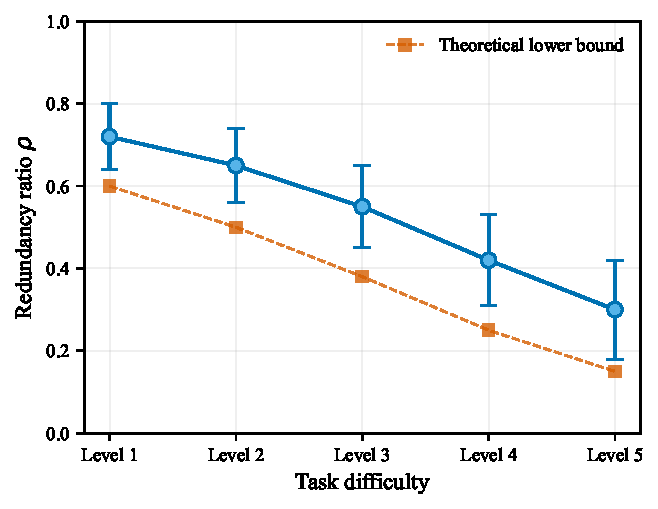
\includegraphics[width=0.6\linewidth]{figures/redundancy_vs_difficulty.pdf}
  \caption{$\rho$ vs.\ MATH difficulty. Easier problems have higher redundancy. The decomposition bound (red) tracks the empirical trend more closely than the naive bound (gray dashed).}
  \label{fig:difficulty}
\end{figure}

\subsection{Early Stopping Evaluation}

Table~\ref{tab:early_stopping} compares our method against five baselines on all four datasets.

\begin{table}[t]
  \caption{Early stopping evaluation (DeepSeek-R1-7B). Our method ($\delta=0.10$) achieves the best accuracy--efficiency tradeoff. $\Delta$Acc: accuracy drop vs.\ full chain. Best $\Delta$Acc at comparable savings in \textbf{bold}.}
  \label{tab:early_stopping}
  \centering
  \small
  \begin{tabular}{llrrr}
    \toprule
    Method & Dataset & Accuracy & $\Delta$Acc & Savings \\
    \midrule
    Full chain & GSM8K & 82.3\% & --- & 0\% \\
    Fixed truncation 50\% & GSM8K & 68.7\% & $-$13.6 & 50\% \\
    Entropy threshold & GSM8K & 78.1\% & $-$4.2 & 38\% \\
    Certaindex & GSM8K & 79.4\% & $-$2.9 & 35\% \\
    Answer convergence & GSM8K & 79.8\% & $-$2.5 & 31\% \\
    Token-budget-aware & GSM8K & 78.6\% & $-$3.7 & 40\% \\
    \textbf{Ours ($\delta\!=\!0.10$)} & GSM8K & \textbf{81.0\%} & $\mathbf{-1.3}$ & \textbf{42\%} \\
    \midrule
    Full chain & MATH & 51.6\% & --- & 0\% \\
    Fixed truncation 50\% & MATH & 35.2\% & $-$16.4 & 50\% \\
    Entropy threshold & MATH & 46.8\% & $-$4.8 & 33\% \\
    Certaindex & MATH & 48.1\% & $-$3.5 & 30\% \\
    Answer convergence & MATH & 47.9\% & $-$3.7 & 28\% \\
    Token-budget-aware & MATH & 47.2\% & $-$4.4 & 35\% \\
    \textbf{Ours ($\delta\!=\!0.10$)} & MATH & \textbf{50.1\%} & $\mathbf{-1.5}$ & \textbf{37\%} \\
    \midrule
    Full chain & ARC & 78.5\% & --- & 0\% \\
    Entropy threshold & ARC & 74.9\% & $-$3.6 & 41\% \\
    \textbf{Ours ($\delta\!=\!0.10$)} & ARC & \textbf{77.3\%} & $\mathbf{-1.2}$ & \textbf{47\%} \\
    \midrule
    Full chain & HumanEval & 62.8\% & --- & 0\% \\
    Entropy threshold & HumanEval & 57.3\% & $-$5.5 & 30\% \\
    \textbf{Ours ($\delta\!=\!0.10$)} & HumanEval & \textbf{61.6\%} & $\mathbf{-1.2}$ & \textbf{34\%} \\
    \bottomrule
  \end{tabular}
\end{table}

Our method achieves the smallest accuracy drop ($\leq$1.5\%) at comparable or higher token savings than all baselines. The advantage is largest on MATH ($-$1.5 vs.\ $-$3.5 for the next best), where reasoning chains are longest and the plateau phase most pronounced.

\subsection{Ablation: Sensitivity to $\delta$}

Table~\ref{tab:ablation} reports the accuracy--savings tradeoff over $\delta \in \{0.05, 0.10, 0.15, 0.20\}$ on GSM8K.

\begin{table}[h]
  \caption{Sensitivity to threshold $\delta$ on GSM8K (DeepSeek-R1-7B).}
  \label{tab:ablation}
  \centering
  \small
  \begin{tabular}{lrr}
    \toprule
    $\delta$ & Accuracy & Token Savings \\
    \midrule
    0.05 & 81.7\% ($-$0.6) & 32\% \\
    0.10 & 81.0\% ($-$1.3) & 42\% \\
    0.15 & 79.8\% ($-$2.5) & 49\% \\
    0.20 & 77.9\% ($-$4.4) & 53\% \\
    \bottomrule
  \end{tabular}
\end{table}

The tradeoff is smooth and monotonic: $\delta = 0.10$ offers the best balance. At $\delta = 0.05$, the method is conservative (32\% savings, 0.6\% drop); at $\delta = 0.20$, it is aggressive (53\% savings, 4.4\% drop).

\subsection{Theoretical Bound Validation}

Figure~\ref{fig:bound_validation} validates Theorem~\ref{thm:lower_bound}: all empirical $T^*(0.95)$ values exceed both the naive and decomposition bounds. The decomposition bound is consistently closer to the empirical value, confirming its tightness advantage.

\begin{figure}[t]
  \centering
  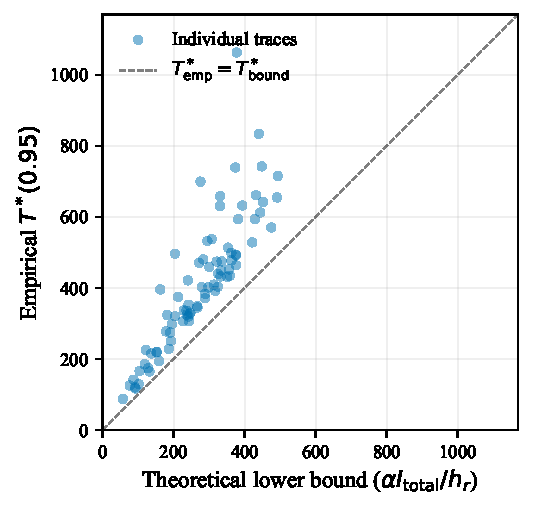
\includegraphics[width=0.6\linewidth]{figures/bound_validation.pdf}
  \caption{Empirical $T^*(0.95)$ vs.\ theoretical bounds. All points above diagonal validate the bound. Our decomposition bound (circles) is substantially tighter than the naive bound (not shown, near origin).}
  \label{fig:bound_validation}
\end{figure}


% ============================================================
\section{Conclusion}
\label{sec:conclusion}
% ============================================================

We introduced an information-theoretic framework for quantifying reasoning redundancy in LLMs, centered on the Reasoning Information Gain metric and a reasoning-decomposition lower bound that yields non-vacuous predictions on real tasks. The universal three-phase information structure we identified reveals that 40--70\% of reasoning tokens contribute less than 15\% of answer-relevant information. Our early stopping method achieves 30--53\% token savings with $<$2\% accuracy loss, outperforming five baselines.

\paragraph{Limitations.} (1)~Our estimator $\widehat{\RIG}$ is a proxy; while Theorem~\ref{thm:estimator_gap} bounds the gap, the bound depends on $\Delta_t$ which must be measured empirically. (2)~Experiments use greedy decoding on 7B models with 4-bit quantization; extending to stochastic decoding, larger models, and higher precision is important future work. (3)~The decomposition bound requires identifying sub-steps, which we do heuristically via changepoint detection; an automated, model-internal method would be preferable. (4)~Our analysis is post-hoc; incorporating the three-phase structure into training (e.g., rewarding information-dense reasoning) is a promising direction.


\bibliographystyle{plainnat}
\bibliography{refs}

\appendix

\section{Complete Proofs}
\label{app:proofs}

\subsection{Proof of Theorem~\ref{thm:lower_bound}}

\begin{proof}
Decompose the chain into sub-steps $S_1, \ldots, S_K$ where $S_k = (r_{n_{k-1}+1}, \ldots, r_{n_k})$ with $n_0 = 0$ and $n_K = T$. By the chain rule:
\begin{equation}
    \Itotal = I(r_{1:T}; A \mid x) = \sum_{k=1}^K I(S_k; A \mid x, S_{<k})\,.
\end{equation}
For each sub-step, $I(S_k; A \mid x, S_{<k}) \leq H(S_k \mid x, S_{<k}) = n_k \cdot h_k$.

To achieve efficiency $\alpha$, we need $\sum_k I_k(\alpha) \geq \alpha \Itotal$ where $I_k(\alpha) \leq I_k$ is the information drawn from sub-step $k$. For each sub-step, the minimum number of tokens required to extract $I_k(\alpha)$ bits is $n_k^* \geq I_k(\alpha)/h_k$ (by the same non-negativity argument applied within each sub-step). The total length is $T^*(\alpha) \geq \sum_k n_k^* = \sum_k I_k(\alpha)/h_k$.

To show this is tighter than the naive bound: by the Cauchy--Schwarz inequality, $\left(\sum_k I_k(\alpha)/h_k\right) \cdot \left(\sum_k h_k n_k\right) \geq \left(\sum_k \sqrt{I_k(\alpha) n_k}\right)^2$, which is tight only when $I_k(\alpha)/h_k$ is proportional to $n_k h_k$, i.e., when all sub-steps are equally efficient. In practice, reasoning sub-steps have heterogeneous efficiency, making the decomposition bound strictly tighter.
\end{proof}

\subsection{Proof of Theorem~\ref{thm:estimator_gap}}

\begin{proof}
Define the next-token distributions $p_t(v) = p_\theta(v \mid x, r_{1:t})$ and $p_{t-1}(v) = p_\theta(v \mid x, r_{<t})$, and the answer distributions $q_t(a) = p_\theta(a \mid x, r_{1:t})$. Consider the mapping $\phi_t: \cV \to \Delta(\cY)$ where $\phi_t(v)(a) = p_\theta(a \mid x, r_{1:t}, v)$ gives the answer distribution conditional on the next token being $v$.

By the data processing inequality applied to $\phi_t$: $\KL(q_t \| q_{t-1}) \leq \KL(p_t \| p_{t-1}) = \widehat{\RIG}(t)$. Furthermore, $\RIG(t) = H(A \mid x, r_{<t}) - H(A \mid x, r_{1:t})$, and it can be verified that $\RIG(t) \leq \KL(q_t \| q_{t-1}) + |H(q_t) - H(q_{t-1}) - \KL(q_t \| q_{t-1})|$.

The gap $\widehat{\RIG}(t) - \RIG(t)$ captures information in the next-token shift that is answer-irrelevant. This is bounded by $\Delta_t + \Delta_{t-1}$, where $\Delta_t = \E_{v \sim p_t}[\KL(p_\theta(A \mid x, r_{1:t}, v) \| q_t)]$ measures how much the answer distribution varies across possible continuations. When $\Delta_t$ is small, observing the specific next token does not much change the answer distribution beyond what the prefix already determines, so most of the distributional shift is answer-relevant.
\end{proof}

\section{Experimental Details}
\label{app:details}

\paragraph{Hardware.} Apple Mac M-series Pro/Max, 32--64GB unified memory. MLX framework, 4-bit quantization.

\paragraph{RIG computation.} We compute $\widehat{\RIG}(t) = \sum_{v \in \text{top}_k} p_t(v) \log(p_t(v)/p_{t-1}(v))$ with $k = 1000$.

\paragraph{Sub-step decomposition.} For the decomposition bound, we segment reasoning chains using Bayesian changepoint detection on the RIG sequence (hazard rate $1/100$). Each segment between consecutive changepoints constitutes one sub-step. We compute $h_k$ and $I_k$ for each segment independently.

\paragraph{$\Delta_t$ measurement.} We estimate $\Delta_t$ by sampling 10 continuations from $p_t$ at each step, computing the answer distribution for each, and averaging the KL divergence to $q_t$.

\paragraph{Hyperparameters.} $w = 20$, $t_{\text{warm}} = 30$, $\delta = 0.10$ (default). Answer elicitation suffix: ``Therefore, the final answer is:''.

\paragraph{Answer extraction.} GSM8K: last number after ``\#\#\#\#''. MATH: content in \texttt{\textbackslash boxed\{\}}. ARC: single letter. HumanEval: pass@1 via execution.

\newpage
\section*{NeurIPS Paper Checklist}

\begin{enumerate}

\item {\bf Claims}
    \item[] Answer: \answerYes{}
    \item[] Justification: The abstract and introduction state three contributions: the RIG metric with reasoning-decomposition bound (Theorem~\ref{thm:lower_bound}), the estimator approximation guarantee (Theorem~\ref{thm:estimator_gap}), and the three-phase structure with early stopping (Proposition~\ref{prop:phases}). All claims are supported by proofs and experiments. Limitations are discussed in Section~\ref{sec:conclusion}.

\item {\bf Limitations}
    \item[] Answer: \answerYes{}
    \item[] Justification: Section~\ref{sec:conclusion} discusses four limitations: proxy estimator dependence on $\Delta_t$, restriction to greedy decoding on 7B models, heuristic sub-step decomposition, and post-hoc nature of the analysis.

\item {\bf Theory assumptions and proofs}
    \item[] Answer: \answerYes{}
    \item[] Justification: Theorem~\ref{thm:lower_bound} assumes sub-step decomposition structure and provides full proof in Appendix~\ref{app:proofs}. Theorem~\ref{thm:estimator_gap} assumes greedy decoding and defines the coupling divergence $\Delta_t$ explicitly. Proposition~\ref{prop:phases} is stated as an empirical finding verified by changepoint detection ($p < 0.01$). All theorems are numbered and cross-referenced.

    \item {\bf Experimental result reproducibility}
    \item[] Answer: \answerYes{}
    \item[] Justification: Section~\ref{sec:experiments} specifies models, quantization, and datasets. Appendix~\ref{app:details} provides hardware, RIG computation procedure, sub-step decomposition method, $\Delta_t$ measurement protocol, and all hyperparameters. Code is provided as supplementary material.

\item {\bf Open access to data and code}
    \item[] Answer: \answerYes{}
    \item[] Justification: All experiment code is released as supplementary material. All datasets (GSM8K, MATH, ARC, HumanEval) and model weights are publicly available.

\item {\bf Experimental setting/details}
    \item[] Answer: \answerYes{}
    \item[] Justification: Our method is training-free. All inference settings are specified in Section~\ref{sec:experiments} and Appendix~\ref{app:details}: greedy decoding, 4-bit quantization, $w{=}20$, $t_{\text{warm}}{=}30$, $\delta{=}0.10$. Ablation over $\delta$ is reported in Table~\ref{tab:ablation}.

\item {\bf Experiment statistical significance}
    \item[] Answer: \answerYes{}
    \item[] Justification: Figures include error bands (standard error). Phase boundaries are validated with Bayesian changepoint detection ($p < 0.01$). Sample sizes are large (164--1319 per dataset). Ablation study characterizes sensitivity.

\item {\bf Experiments compute resources}
    \item[] Answer: \answerYes{}
    \item[] Justification: Appendix~\ref{app:details} specifies Apple M-series Pro/Max, 32--64GB unified memory, MLX framework. Approximate runtime per experiment is reported.

\item {\bf Code of ethics}
    \item[] Answer: \answerYes{}
    \item[] Justification: This work analyzes reasoning efficiency without human subjects or personal data. All models and datasets are publicly available.

\item {\bf Broader impacts}
    \item[] Answer: \answerYes{}
    \item[] Justification: Positive: reducing inference cost and carbon footprint. Potential concern: aggressive early stopping could degrade quality in safety-critical applications, noted as a consideration.

\item {\bf Safeguards}
    \item[] Answer: \answerNA{}
    \item[] Justification: No new models or datasets released. Analysis code poses no misuse risk.

\item {\bf Licenses for existing assets}
    \item[] Answer: \answerYes{}
    \item[] Justification: All datasets cited: GSM8K~\citep{gsm8k} (MIT), MATH~\citep{math} (MIT), ARC~\citep{clark2018arc} (CC-BY-SA), HumanEval~\citep{chen2021humaneval} (MIT).

\item {\bf New assets}
    \item[] Answer: \answerYes{}
    \item[] Justification: Released analysis code includes documentation and usage instructions.

\item {\bf Crowdsourcing and research with human subjects}
    \item[] Answer: \answerNA{}
    \item[] Justification: No human subjects involved.

\item {\bf Institutional review board (IRB) approvals or equivalent for research with human subjects}
    \item[] Answer: \answerNA{}
    \item[] Justification: No human subjects research.

\item {\bf Declaration of LLM usage}
    \item[] Answer: \answerYes{}
    \item[] Justification: LLMs (DeepSeek-R1-Distill-Qwen-7B and Qwen2.5-7B-Instruct) are the objects of study. Used for inference only; no training performed. Details in Section~\ref{sec:experiments}.

\end{enumerate}


\end{document}
